\documentclass[mathserif]{beamer}
\usepackage{beamerthemeshadow}
\usepackage{beamerthemesplit}
%\usetheme{shadow}
\usecolortheme{default}
\setbeamertemplate{footline}[frame number]
\useinnertheme[shadow=true]{rounded}
%\setbeamertemplate{footline}{\insertframenumber/\inserttotalframenumber}
%\useoutertheme{infolines}
%\setbeamertemplate{headline}{} % removes the headline that infolines inserts

%\usetheme{boxes}
%\usepackage{amsmass}
%\usepackage{amssymb,amsfonts,url}


\usepackage{algorithm}
\usepackage{algorithmic}

\usepackage{graphicx}
\graphicspath{{Problems/}}


%\usepackage{CJK}
%\usepackage{pinyin}

%    \begin{figure}
%        \centering
%        \includegraphics[width=0.8\textwidth]{newGeneRep.eps}
%    \end{figure}

% \begin{figure}%
%   \begin{center}%
%     \begin{minipage}{0.70\textwidth}%
%      \includegraphics[width=1.0\textwidth]{comp25000.eps}%
%     \end{minipage}%
%     \begin{minipage}{0.30\textwidth}
%      \includegraphics[width=1.0\textwidth]{comparelabel.eps}%
%     \end{minipage}%
%   \end{center}
% \end{figure}

% \begin{table}
%   {\begin{tabular}{l|rrr}\hline
%       & \multicolumn{3}{c}{Actual number of DCJ operations}\\
%       \# genes &\# genes $\times 1$&\# genes $\times 2$&\# genes  $\times 3$ \\
% \hline
%      (a)~25,000 & 0.5\% ~~&  0.9\% ~~& 1.7\%~~\\
%       (b)~10,000 & 0.8\%~~ &  1.4\% ~~& 2.7\%~~\\
%      (c)~ 1,000 & 2.7\%~~ & 4.7\%~~ & 14.7\%~~\\ \hline
%     \end{tabular}} {}%
% \end{table}

% \begin{eqnarray}
% T(n) &=&  \sum_{i=1}^n C_i \\
%      &=&  \# PUSH + \#POP \\
%      &<& 2\times \#PUSH \\
%      &<& 2n \\
% \end{eqnarray}


\title{CS711008Z Algorithm Design and Analysis }
\subtitle{ Lecture 5. Fast Division \footnote{The slides are prepared based on Lecture 30 of The Design and Analysis of Algorithms (by D. C. Kozen) } }
\author{Dongbo Bu \\
\ \ \ \ \ \ \ \ \ \ \ \ \ \ \ \ \ \ \ \ \ \ \ \ \ \ \ \ \ \ \ \ \ \ \ \ \ \ \ \ \ \ \ \ \ \ \ \ \ \ \ \ \ \ \ \ \ \ \ \ \ \ \ \ \ \ \ \ \ \ \ \ \ \ \ \ \ \ \ \ \ \ \ \ \ \ \ \ \ \ \ \ \ \ \ \ \ \ \ \  \\
{\small Institute of Computing Technology \\ Chinese Academy of Sciences, Beijing, China}}
\date{}


\begin{document}
%\begin{CJK}{UTF8}{cyberbit}

\maketitle 

\frame{
\frametitle{ {\sc Fast Integer Division} }
\begin{block}{} 
{\bf Input: } Two integers numerator (also called dividend)  $n$ and denominator  (also called divisor )$d$ with at most $k$ bits;  \\
{\bf Output: } Two integers quotient $q$ and remainder $r$ such that $q= n / d$ and $r = n \mod d$. 
\end{block} 
} 
 
\frame{
	\frametitle{Two types of division algorithms} 
	Division algorithms fall into two main categories: 
	\begin{itemize}
		\item Slow division algorithms:  producing one digit of the final quotient per iteration.
		\item Fast division algorithms:  starting with a close approximation to the final quotient, and producing twice as many digits of the final quotient on each iteration.
	\end{itemize}
}
 
\frame{
\frametitle{ Grade school algorithm: {\sc Long Division}  } 	
	\begin{figure}
		 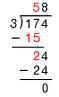
\includegraphics[width=1in] {L5-long-division.eps}
	\end{figure}
\begin{itemize}
	\item Generating a digit at each iteration
	\item Time-complextiy: $O(k^{2})$ addition
 	\item Question:  Is grade school algorithm optimal? 
\end{itemize}
}


 
\frame{
\frametitle{ {\sc Fast Division} }
\begin{itemize}
 \item Problem: Given two $n$-digit numbers $s$ and $t$, to calculate $q=s/t$ and $r = s \mod t$. 
 \item Methods: 
 \begin{enumerate}
  \item Calculate $ x = 1 / t$ using Newton's method first: $x_{i+1} =  2 x_i - t \times x_i^2 $.
  \item At most $\log n $ iterations are needed. 
  \item Thus division is as fast as multiplication.
 \end{enumerate}
\end{itemize}
}



\frame{
\frametitle{Details of {\sc Fast Division}: Newton's method }
Objective: Calculate $x=1/t$.  
\begin{itemize}
 \item $x$ is the root of $f(x) = 0$, where $f(x) = (t - \frac{1}{x})$. (Why
 the form here?)
 \item Newton's method: 
 \begin{eqnarray}
 x_{i+1} &=& x_i - \frac{f(x_i)}{f'(x_i)} \\
         &=& x_i - \frac{t-\frac{1}{x_i}}{ \frac{1}{x_i^2} } \\
         &=& - t\times x_i^2 + 2 x_i 
 \end{eqnarray}
 \item Convergence speed: quadratic, i.e. $\epsilon_{i+1} \leq M \epsilon_i^2$,
 where $M$ is a supremum of a ratio, and $\epsilon_i$ denotes the distance between $x_i$  and $\frac{1}{t}$. Thus the number of iterations is limited by  $\log \log t = O(\log n)$.
\end{itemize}
}


\frame{
\frametitle{ {\sc Fast Division}: an example }

Objective: to calculate $\frac{1}{13}$. 
\begin{center} 
\begin{tabular}{ l c c } 
\hline \\
\#Iteration & $x_i$ & $\epsilon_i$ \\ 
\hline 
 0	&0.0187	&-0.0582231 \\
1	&0.032854	&-0.044069  \\
2	&0.051676	&-0.0252471 \\
3	&0.0686367	&-0.00828638 \\
4	&0.0760304	&-0.000892633 \\
5	&0.0769127	&-1.03583e-05 \\
6	&0.0769231	&-1.39483e-09 \\
7	&0.0769231	&-2.77556e-17 \\
8	&0.0769231	&0 \\
 \hline
\end{tabular}
\end{center} 
Note: the quadratic convergence implies that the error $\epsilon_i$ has a form of $O(e^{2^i})$; thus the iteration number is limited by $\log \log (t)$. 
}


\end{document}
